\documentclass{article}

\usepackage[english]{babel}
\usepackage{float}
\usepackage[letterpaper,top=2cm,bottom=2cm,left=3cm,right=3cm,marginparwidth=2cm]{geometry}
\usepackage{amsmath}
\usepackage{amssymb}
\usepackage{graphicx}
\usepackage{grffile}
\usepackage{booktabs}
\usepackage{array}
\usepackage{tabularx}
\usepackage{caption}
\usepackage{verbatim}
\usepackage{xcolor}
\usepackage{fancyvrb}
\usepackage{tikz}
\usetikzlibrary{arrows.meta, positioning, calc}
\captionsetup[figure]{justification=centering}
\usepackage[colorlinks=true, allcolors=blue]{hyperref}
\setlength{\emergencystretch}{3em}

\title{\textbf{ME 144L Lab Prelab 10: PMDC Motor Speed Control}}
\author{Alejandro Diaz \\ TA: Gabrielle Naquila}
\date{April 14, 2026}

\begin{document}
\maketitle

% =======================================================
\section{Motor Parameters and Simulation Setup}
% =======================================================

The provided \texttt{pmdc\_motor\_OL\_sim.py} drives the motor model at a user-specified speed $\omega_d$ by inverting the steady-state torque-speed relation for the required armature voltage, then converting that voltage to a PWM command. The key equations are:
\begin{equation}
    V_{in}(\omega_d)
    \;=\; r_m\,\omega_d
    \;+\; \frac{R_m}{r_m}\!\left[\,B_m\,\omega_d \;+\; \tau_{mo}\tanh(\omega_d)\,\right]
    \label{eq:ol_vin}
\end{equation}
\begin{equation}
    \mathrm{PWM}(\omega_d) \;=\; 255 \cdot \frac{V_{in}(\omega_d)}{V_b}
    \label{eq:ol_pwm}
\end{equation}

\noindent Table 1 lists the motor parameters, which were extracted from Lab 9 testing, and the bus voltage matches the supply used in Lab 9.
\begin{table}[H]
    \centering
    \caption{Motor Parameters from Lab 9 Testing.}
    \label{tab:params}
    \begin{tabular}{llc}
        \toprule
        Symbol & Name & Value \\
        \midrule
        $r_m$      & Motor constant                 & $1.011\cdot 10^{-2}~\mathrm{V\!\cdot\!s/rad}$ \\
        $R_m$      & Armature resistance            & $26.9~\Omega$ \\
        $B_m$      & Viscous damping                & $4.71\cdot 10^{-7}~\mathrm{N\!\cdot\!m\!\cdot\!s/rad}$ \\
        $\tau_{mo}$& Coulomb friction torque        & $9.81\cdot 10^{-5}~\mathrm{N\!\cdot\!m}$ \\
        $GR$       & Gearbox reduction              & 45 \\
        $J_m$      & Rotational inertia  & $1.45\cdot 10^{-7}~\mathrm{kg\!\cdot\!m^2}$ \\
        $V_b$      & Bus voltage                    & $4.82~\mathrm{V}$ \\
        \bottomrule
    \end{tabular}
\end{table}

% =======================================================
\section{PWM Subplotting}
% =======================================================

The first figure in the provided script originally had three stacked plots: input voltage, motor speed with the reference overlay, and speed error. To build a PWM trace above the voltage trace, the edit to \texttt{pmdc\_motor\_OL\_sim.py} is small, storing \texttt{PWM[i] = mcc*255} in the loop and add a fourth axis at the top of the subplot stack. Figure 1 shows the four-subplot output for the middle test case, $\omega_d = 212.59~\mathrm{rad/s}$. The PWM pulse and $V_{in}$ switch on together at $t = 0.1~\mathrm{s}$. The speed reaches its reference quickly because the rotor time constant is much faster than $dt$.

\begin{figure}[H]
    \centering
    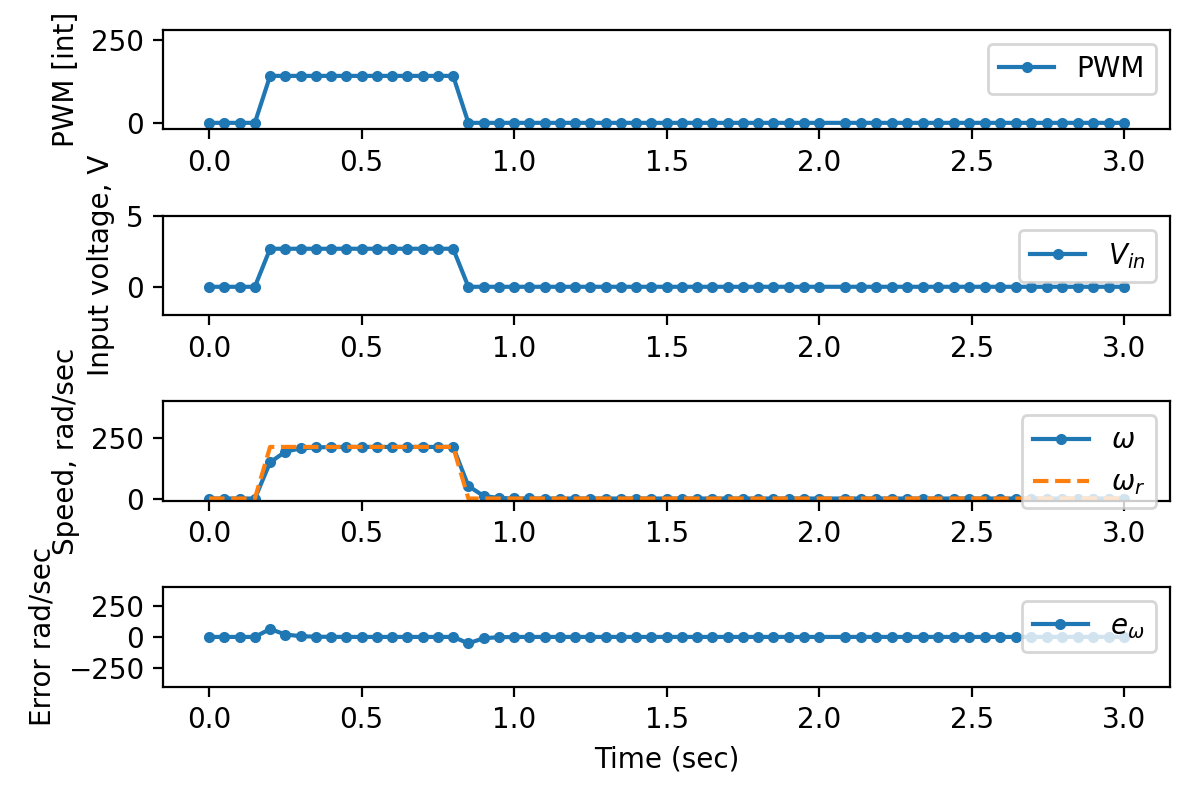
\includegraphics[width=0.75\linewidth]{images/ol_sim_w2030rpm.png}
    \caption{Four-subplot output of the modified open-loop simulation at $\omega_d = 212.59~\mathrm{rad/s}$ (2030~RPM). From top to bottom: commanded PWM, input voltage, motor speed with reference overlay, and speed error.}
    \label{fig:ol_sim_mid}
\end{figure}

% =======================================================
\section{Three-Point Comparison Against Lab 9 Experimental Data}
% =======================================================

Three operating points from Lab 9 are used as desired speeds. Table 2 and Figure 2 summarize the results.

\begin{table}[H]
    \centering
    \caption{Open-loop sim vs. Lab 9 measurements. $\omega_d$ is the desired motor-shaft speed, $\omega_{ss}^{\text{sim}}$ is the simulated steady-state speed after ODE integration, and percent differences are referenced to the experimental value.}
    \label{tab:compare}
    \begin{tabular}{ccccccc}
        \toprule
        $\omega_d$~[rad/s] & RPM & $\mathrm{PWM}_{\text{exp}}$ & $\mathrm{PWM}_{\text{sim}}$ & $\omega_{ss}^{\text{sim}}$~[rad/s] & $\Delta \mathrm{PWM}$ & $\Delta \omega$ \\
        \midrule
        340.34 & 3250 & 230 & 218.4 & 340.34 & $-5.04\%$ & $\phantom{+}0.00\%$ \\
        212.59 & 2030 & 155 & 141.6 & 212.62 & $-8.64\%$ & $+0.02\%$ \\
         90.06 &  860 &  80 &  68.0 &  92.10 & $-15.06\%$ & $+2.26\%$ \\
        \bottomrule
    \end{tabular}
\end{table}

\begin{figure}[H]
    \centering
    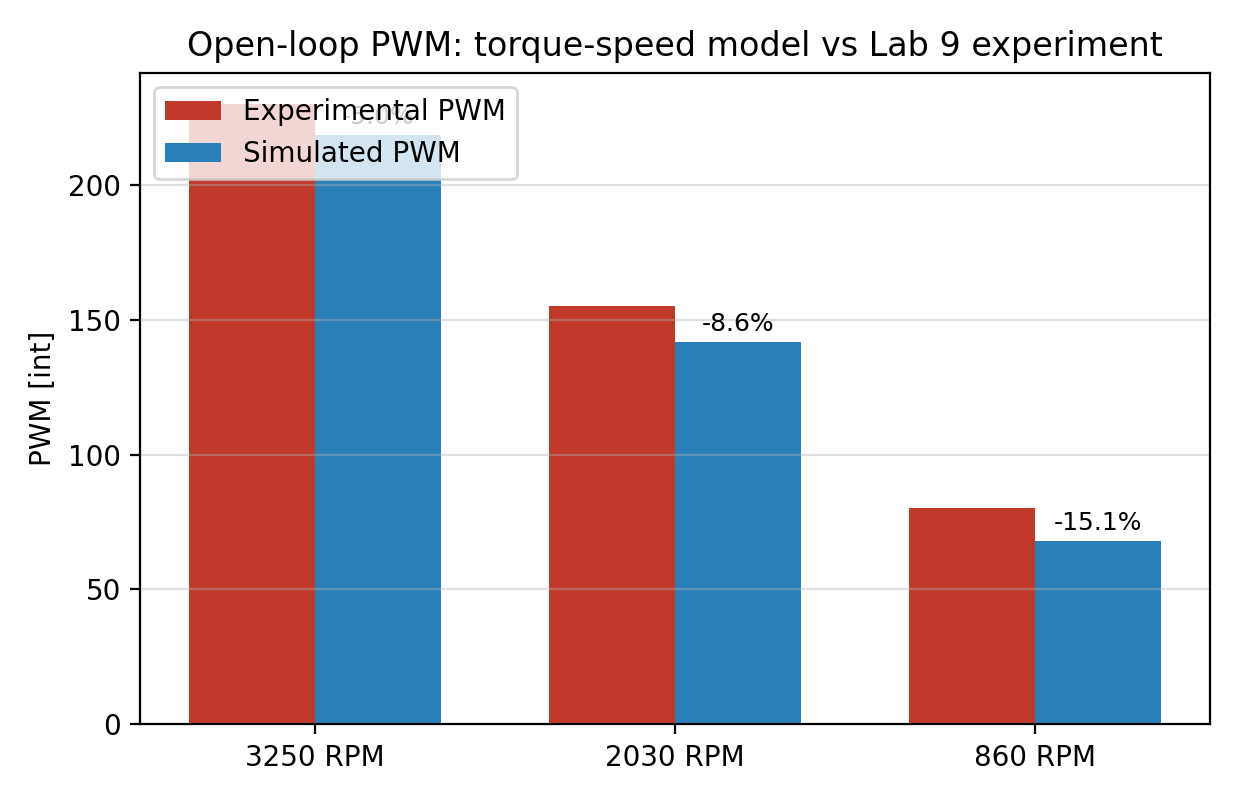
\includegraphics[width=0.65
    \linewidth]{figures/sim_vs_exp_pwm.png}
    \caption{PWM from the torque-speed model vs the PWM measured in Lab 9 at equal speed.}
    \label{fig:pwm_bars}
\end{figure}

\noindent The simulated speed matches the desired speed within $2.3\%$ across all three points. The PWM error grows as speed drops, indicating $-5.0\%$ at 3250~RPM, $-8.6\%$ at 2030~RPM, and $-15.1\%$ at 860~RPM. The torque-speed model does not account for friction losses well at low speed, requiring less PWM than the motor required in the experiment.

% =======================================================
\section{Closed-Loop Feedback Control Diagram}
% =======================================================

A closed-loop speed controller measures the actual motor speed, subtracts it from the reference to form an error, and feeds that error through a controller that outputs the PWM. Figure 3 represents the speed control system as a block diagram.

\begin{figure}[H]
    \centering
    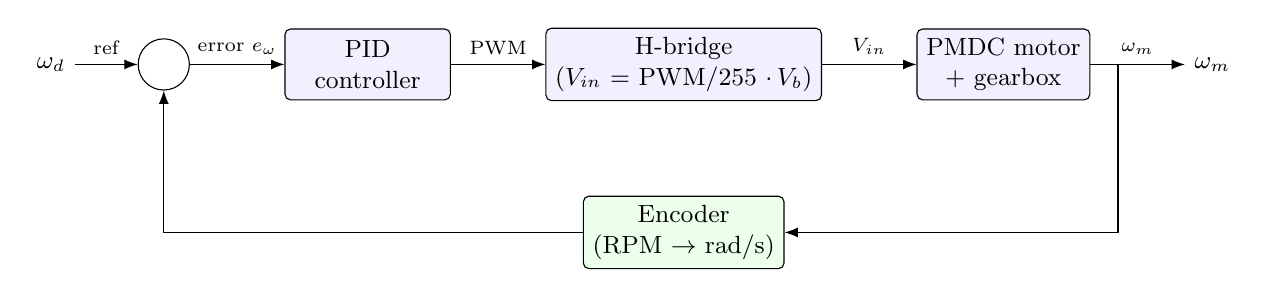
\begin{tikzpicture}[
        node distance=1.4cm and 1.2cm,
        block/.style={draw, rectangle, rounded corners=2pt, minimum width=2.1cm, minimum height=0.9cm, align=center, fill=blue!6},
        sum/.style={draw, circle, minimum size=0.65cm, inner sep=0pt},
        sensor/.style={draw, rectangle, rounded corners=2pt, minimum width=2.1cm, minimum height=0.8cm, align=center, fill=green!8},
        >=Latex,
        font=\small,
    ]
        \node (ref)  at (0,0)                       {$\omega_d$};
        \node[sum,   right=0.8cm of ref]     (sum) {};
        \node[block, right=of sum]          (ctrl) {PID\\controller};
        \node[block, right=of ctrl]         (drv)  {H-bridge\\($V_{in}$ = PWM/255 $\cdot\,V_b$)};
        \node[block, right=of drv]          (plant){PMDC motor\\+ gearbox};
        \node       [right=1.2cm of plant]  (out)  {$\omega_m$};
        \node[sensor, below=1.2cm of drv]   (enc)  {Encoder\\(RPM $\to$ rad/s)};

        \draw[->] (ref)    -- (sum) node[midway, above] {\scriptsize ref};
        \draw[->] (sum)    -- (ctrl) node[midway, above] {\scriptsize error $e_\omega$};
        \draw[->] (ctrl)   -- (drv)  node[midway, above] {\scriptsize PWM};
        \draw[->] (drv)    -- (plant) node[midway, above] {\scriptsize $V_{in}$};
        \draw[->] (plant)  -- (out)  node[midway, above] {\scriptsize $\omega_m$};
        \draw[->] ($(plant.east)+(0.35,0)$) |- (enc);
        \draw[->] (enc)    -| (sum);
    \end{tikzpicture}
    \caption{Closed-loop speed controller for the PMDC motor. The reference speed $\omega_d$ is compared against the encoder reading, the PID block converts the speed error $e_\omega$ into a PWM command, the H-bridge converts that command into an armature voltage, and the motor/gearbox plant produces the measured shaft speed. (Diagram formalized in \texttt{tikz} with assistance from Claude Opus 4.6.)}
    \label{fig:cl_diagram}
\end{figure}

\subsection{Advantages of closing the loop}

\noindent Closing the loop mainly helps where the open-loop model falls short. The integral term picks up the PWM gap from Table 2 on its own, so there is no need to re-characterize the motor each time conditions change. Supply voltage drifts, load spikes, and friction from temperature all get corrected without touching the model. Swapping a motor is easier too since tuning the gains is faster than redoing the full bench test.

\subsection{Disadvantages of closing the loop}

\noindent Some key disadvantages are that dead encoders means there is nothing to feed back, so the whole point of the controller is gone. $K_p$, $K_i$, $K_d$, and the sample rate all interact, so getting them right takes iteration. Integrator windup is also something to watch for: if the PWM command sits at $\pm 255$ long enough, the integral accumulates and the motor overshoots when it comes back into range.

\end{document}
